\section{Bussysteme}
Bei einem Bussystem teilen sich mehrere Teilnehmer (z.B. Arduinos) einen Übertragungsweg.

\textbf{Grundlegende Eigenschaften} \\
\begin{itemize}
	\item Übertragungsart
	\begin{itemize}
		\item Seriell: Zeichen werden nacheinander übertragen
		\item Parallel: Zeichen werden gleichzeitig übertragen
	\end{itemize}
	\item Topologie
	\begin{itemize}
		\item Punkt-zu-Punkt
		\item Linientopologie
		\item Sterntopologie
		\item Ringtopologie
		\item Baumtopologie
		\begin{figure}[H]
			\centering
			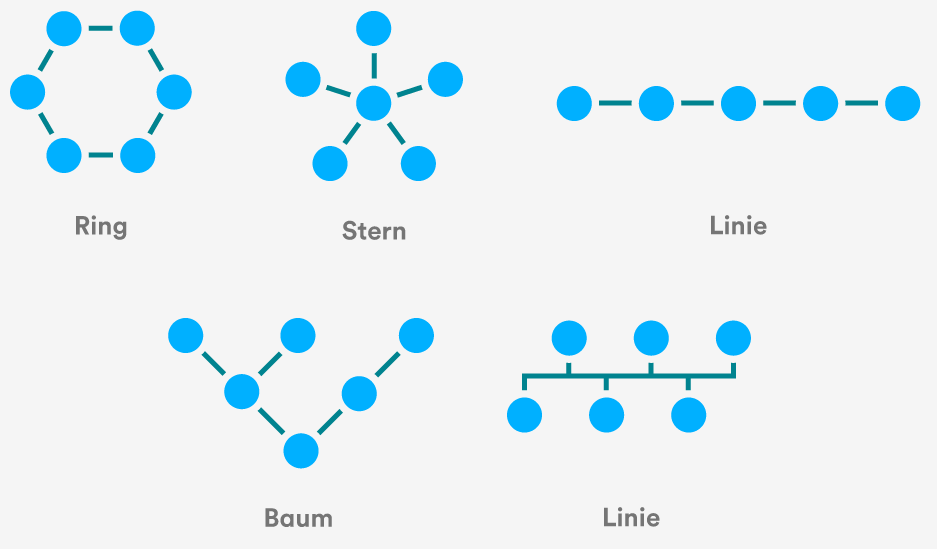
\includegraphics[width=0.7\linewidth]{figures/topo.png}
			\caption{Bustopologiearten}
		\end{figure}
	\end{itemize}
	\item Priorisierung, Kollisionsvermeidung
	\item Synchronisierung
	\begin{itemize}
		\item synchron: eigene Taktleitung
		\item asynchron: keine Taktleitung, fix vorgegebene Übertragungsrate \\
		Einheit: 1 baud = 1 $\dfrac{\text{bit}}{\text{s}}$
	\end{itemize}
	\item Fehlererkennung
\end{itemize}

Konkrete Beispiele: RS-232, CAN, I2C, SPI, USB, Bluetooth

\subsection{RS-232 (UART)}
RS-232 kann zwei Geräte miteinander verbinden.
\begin{itemize}
	\item Topologie: Punkt-zu-Punkt
	\item Priorisierung, Kollisionsvermeidung: nicht nötig (2 Kabel: 1x Rx, 1x Tx)
	\item Synchronisierung: asynchron
	\item \begin{tabbing}
		Übertragungsart: Seriell ~~~ \= 3 bis 15V '1' \\
		~~~~~~~~~~~~~~~~~~~~~~~~~~~~~~~~ \= -3 bis -15V '0'
	\end{tabbing}
	Achtung: Alle Arduinos nutzen den gleichen GND-Pin!
	\item Fehlererkennung: eventuell mit einem Parity-Bit
\end{itemize}

\textbf{Konkrete Umsetzung} \\
Beim RS-232 bestehen die Daten aus einem Startbit, 5-8 Datenbits, dann eventuell ein Parity-Bit und am Ende 1 bis 2 Stopbits

Bsp: 9600 8E1 \\
\begin{tabular}{c|c|c|c}
	9600&8&E&1 \\
	\hline
	Übertragungswert&Anzahl der Datenbits&ein Even-Parity-Bit&Anzahl der Stoppbits \\
\end{tabular}


'a' ASCII, 97 $\rightarrow$ 011 0000 1 \\
\begin{tabular}{c|c|c|c}
	0 & 01100001 & 1 & 1 \\
	\hline
	Start & Datenbits & Parity-bit & Stopp-Bit \\
\end{tabular}

Das Parity-Bit kann
\begin{itemize}
	\item O ... Odd
	\item E ... Even
	\item N ... None
\end{itemize}
sein

Bsp 2: 96000 8O1 \\
'S', 83 $\rightarrow$ 1010011 \quad 0 1010011 1 1 \\
'E', 69 $\rightarrow$ 01000101 \quad 0 1000101 0 1

\textbf{UART am Arduino} \\
Der Arduino besitzt ein UART-Bauteil, welches für die aktuelle Kommunikation genutzt werden kann. UART-Bauteil sendet immer mit 8 Datenbits und immer mit einem Stoppbit.


\textbf{Serial Funktionen} \\
\texttt{Serial.available()} ... wandelt eingegebene Zeichen in ASCII-Zeichen/Zahlen um \\
Beispiel mit Ausgabe: HELLO $\rightarrow$ 72 69 76 76 79 10

\texttt{Serial.print()} ... gibt Daten im Serial Monitor aus
\begin{tabbing}
	z.B. \= \texttt{Serial.print(78)} $\rightarrow$ 78 \\
	~~~~~ \= \texttt{Serial.print("Test")} $\rightarrow$ Test 
\end{tabbing}
Weiters kann man Zahlen in anderen Zahlensystemen umwandeln und ausgeben (BIN, OCT, DEC, HEX) 
\begin{tabbing}
	z.B. \= \texttt{Serial.print(78, BIN)} $\rightarrow$ 1001110 \\
	~~~~~ \= \texttt{Serial.print(78, HEX)} $\rightarrow$ 4E 
\end{tabbing}
oder auch auf Nachkommastellen runden:
\begin{tabbing}
	z.B. \= \texttt{Serial.print(1.23456, 0)} $\rightarrow$ 1 \\
	~~~~~ \= \texttt{Serial.print(1.23456, 2)} $\rightarrow$ 1.23 \\
	~~~~~ \= \texttt{Serial.print(1.23456, 4)} $\rightarrow$ 1.2345
\end{tabbing}

\texttt{Serial.println()} ... gleich wie \texttt{Serial.print()}, jedoch beginnt es mit ASCII 13 oder '\textbackslash r' (neue Zeile beginnen) und endet mit ASCII 10 oder '\textbackslash n' (Zeil beenden).

\texttt{Serial.read()} ... gleich wie Serial.available()

\texttt{Serial.write()} ... ähnlich wie \texttt{Serial.print()} und \texttt{Serial.available()} jedoch wird hier ASCII-Zahlen in Buchstaben umgewandelt.
\begin{tabbing}
	z.B. \= \texttt{Serial.write(72)} $\rightarrow$ H \\
	~~~~~ \= \texttt{Serial.write(69)} $\rightarrow$ E \\
	~~~~~ \= \texttt{Serial.write(76)} $\rightarrow$ L \\
	~~~~~ \= \texttt{Serial.write(76)} $\rightarrow$ L \\
	~~~~~ \= \texttt{Serial.write(79)} $\rightarrow$ O \\
	~~~~~ \= \texttt{Serial.write(32)} $\rightarrow$ SPACE \\
\end{tabbing}


\subsection{CAN-Bus (Controll Area Network)}
Der CAN-Bus ist ein serieller Bus der speziell für die Automobilindustrie entwickelt wurde

\textbf{Aktuelle Anwendungen} \\
\begin{itemize}
	\item Autos (Vernetzung von Steuergeräten und Sensoren)
	\item Flugzeuge
	\item Raumfahrt
	\item Medizintechnik
	\item ...
\end{itemize}
Der CAN-Bus arbeitet nach dem Multi-Master-Prinzip und bildet eine Linientopologie. \\
\textbf{Aufbau}
\begin{figure}[H]
	\centering
	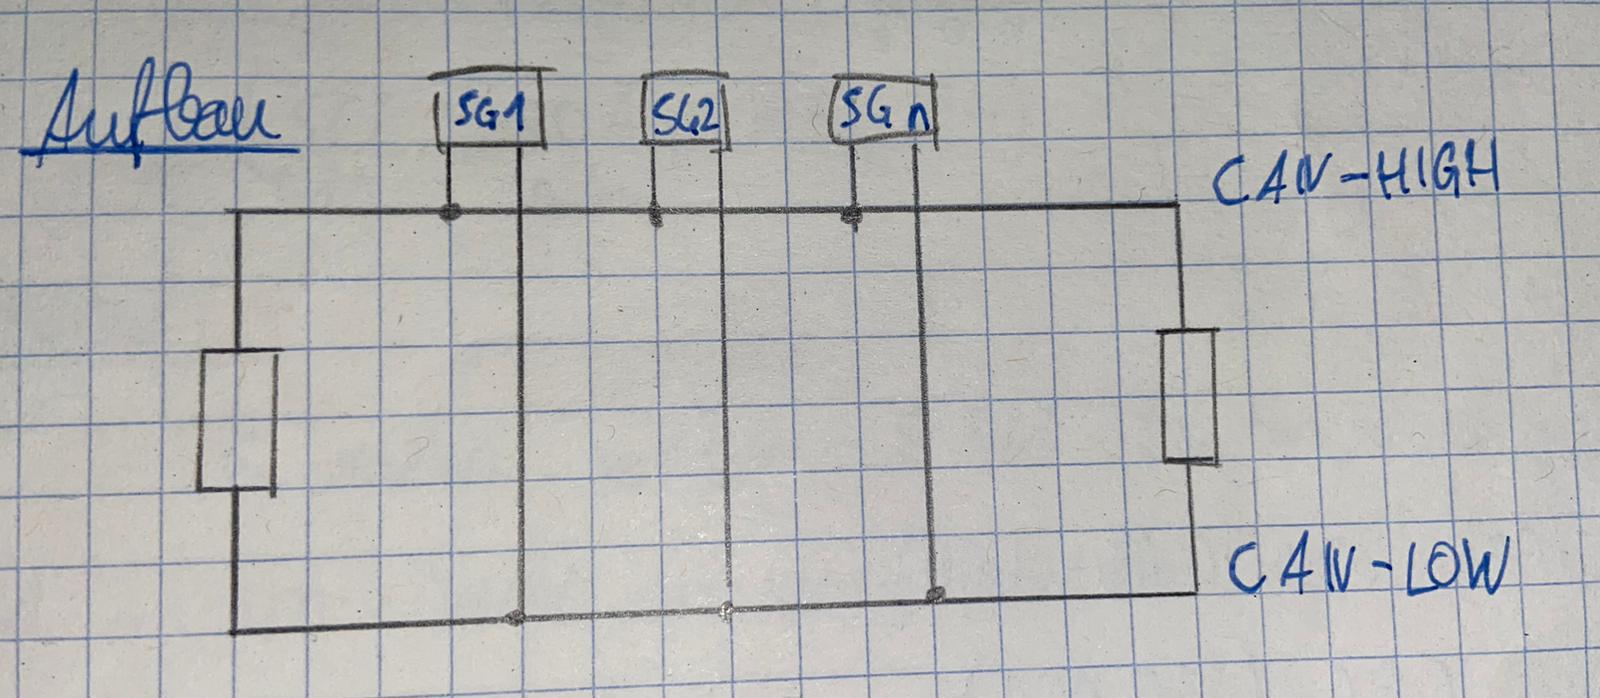
\includegraphics[width=0.8\linewidth]{figures/canbus.jpeg}
	\caption{CAN-Bus Aufbau}
\end{figure}
Der CAN-Bus ist ein asynchroner Bus \\
\begin{tabular}{ccccccc}
	Datenwert & Startbit & 1 & \checkmark && Startbit & 1 \\
	& Message ID & 11 & $\leftarrow$ && Daten & 8 \\
	& Steuerbits & 7 & \checkmark && (Parity & 1) \\
	& Datenbits & 0-64 & \checkmark && Stopp & 1 \\
	& Fehlererkennung & 15 & $\leftarrow$ &&  &  \\
	& Steuerbits & 3 & \checkmark &&  &  \\
	& Stoppbits & 7 & \checkmark &&  &  \\
\end{tabular}

\textbf{Message ID} \\
Dort steht um welche Art von Nachricht es sich handelt und wie wichtig die Nachricht ist (z.B. Wasser, Öl, Airbag). Desto kleiner die Message ID ist, desto wichtiger ist die Nachricht. Jedes Sg kann nur eine Message ID aussenden (Priorisierung).

\textbf{Kollisionsvermeidung CSMA/CR} \\
SG1: M-ID = 000100 \\
SG2: M-ID = 011011 \\
SG3: M-ID = 001101 \\
0 ... dominant \\
1 ... rezessiv

\textbf{Sicherheit} \\
\begin{itemize}
	\item zwei Leitungen (CAN-LOW, CAN-HIGH)
	\item Fehlererkennung mit CRC (15 Bit)
	\item Stuffbit (Stopfbit) Bei fünf gleichen Bits wird ein anderes eingefügt \\
	0000000 \\
	00000100
\end{itemize}

\textbf{Zusammenfassung} \\
\begin{itemize}
	\item seriell
	\item Message ID mit CSMA/CR
	\item Linientopologie
	\item asynchron
	\item Stuffbit, CRC, 2 Leitungen
\end{itemize}

\subsection{I2C-Bus (IIC, I²C)}
Der I2C-Bus wurde Anfang 80er Jahre von der Firma Philips entwickelt. \\
Der I2C-Bus ...
\begin{itemize}
	\item ... ist seriell
	\item ... hat 2 Leiter: SCL \& SDA (Serial Clock, Serial Data)
	\item ... ist synchron
	\item ... funktioniert nach Master-Slave-Prinzip. \\
	Es gibt einen Master (es wären mehrere möglich) $\rightarrow$ keine Kollisionen, Priorisierung unnötig durch Master
\end{itemize}

\textbf{Aufbau} \\
\begin{itemize}
	\item Linientopologie
	\item 2 Leitungen mit Pullup-Wiederstände $\rightarrow$ Ruhe zustand HIGH (SCL Takt, SDA Daten; A5, A4)
\end{itemize}

\textbf{Ablauf} \\
\begin{itemize}
	\item es werden immer 8 Bit Datenwerte gesendet
	\item um Daten zu senden muss der Pegel der Datenleitung stabil sein (0 oder 1), falls die Taktleitung auf HIGH ist. Sobald die Taktleitung auf LOW ist, kann die Datenleitung das Bit setzen.
	\begin{figure}[H]
		\centering
		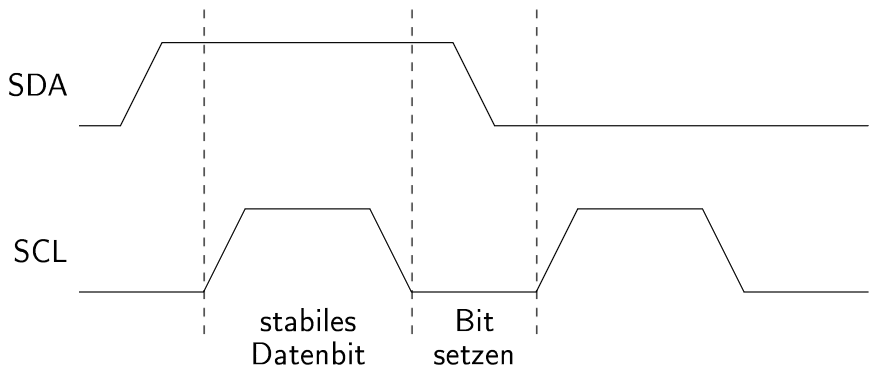
\includegraphics[width=0.8\linewidth]{figures/i2c2.png}
		\caption{I2C-Bus Bitsetzung}
	\end{figure}
	\item Steuersignale
	\begin{itemize}
		\item Startsignal (fallende Flanke, während der Takt auf HIGH ist)
		\item Stopsignal (steigende Flanke, während der Takt auf HIGH ist)
		\begin{figure}[H]
			\centering
			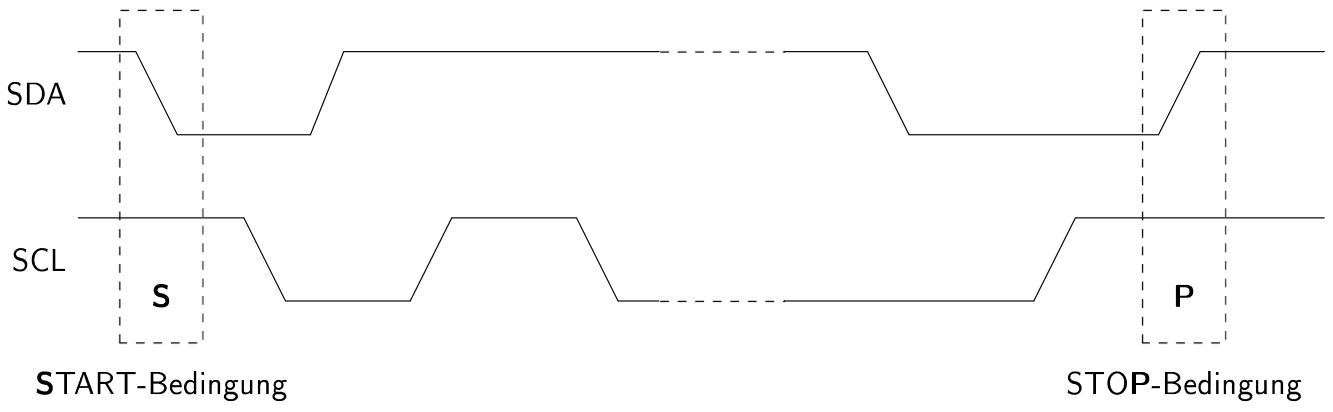
\includegraphics[width=0.8\linewidth]{figures/i2c3.png}
			\caption{I2C-Bus Steuersignale}
		\end{figure}
	\end{itemize}
\end{itemize}

\textbf{Adressierung}
\begin{itemize}
	\item 7 Bit-Adressen für die Slaves \\
	$\rightarrow$ 128 mögliche Teilnehmer (eig. 112)
	\item 0000000 $\rightarrow$ general call address (Broadcastaddresse)
	\item Das 8te Bit sagt ob der Master lesen oder schreiben soll
\end{itemize}

\begin{figure}[H]
	\centering
	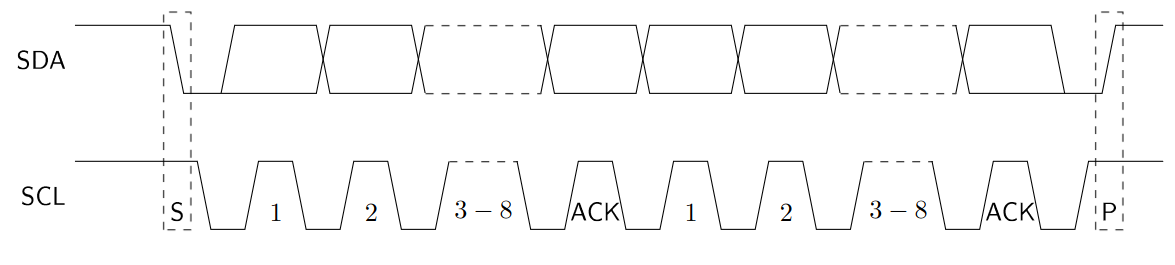
\includegraphics[width=0.8\linewidth]{figures/i2cablauf.png}
	\caption{I2C Ablauf}
\end{figure}

\textbf{Zusammenfassung}
\begin{itemize}
	\item seriell
	\item Linientopologie
	\item Master-Slave $\rightarrow$ unnötig (bei einem Master)
	\item synchron
	\item ACK, Takt
\end{itemize}

\begin{tabular}{ | p{\dimexpr 0.5\linewidth-2\tabcolsep} | p{\dimexpr 0.5\linewidth-2\tabcolsep} |} \hline
	\textbf{Master} & \textbf{Slave} \\ \hline
	\texttt{Wire.beginTransmission(address);} & \texttt{Wire.begin(address);} \\
	\texttt{Wire.endTransmission();} & \texttt{Wire.onRecieve();} \\
	\texttt{Wire.read();} & \texttt{Wire.onRequest();} \\
	\texttt{Wire.write();} &  \\
	\texttt{Wire.available();} &  \\
	\hline
\end{tabular} 

\textbf{I2C-Display (OLED)} \\
Bibliotheken installieren: GFX, SSD 1306 (Adafruit), BusIO \\
Wire $\rightarrow$ I2C Scanner (Adresse auslesen) \\
SSD 1306 $\rightarrow$ 128x64 I2C 

\textbf{OOP am Arduino (C++)} \\
Objekt besteht aus
\begin{itemize}
	\item Attribute, Felder, Eigenschaften
	\item Konstruktor
	\item Funktionen/Methoden
\end{itemize}











